
\chapter{Conclusion}\label{chap:conclusion}


Bayesian methods provide a powerful framework for quantifying uncertainty in ozone
combustion applications. Bayesian calibration, given a set of experimental data of flame speed to compare
against, both improves calibration of the chemical kinetic parameter as well as providing
updated distributions for the parameters. Those distributions can then be
propagated forward into simulations of laminar flame speed to determine the uncertainty in
their predictions. The application of this approach to existing experimental data of flame speed for ozone combustion model was done here.


 We have considered one dimensional flow and used Bayesian inference to infer the chemical parameters involved in the reaction. We have considered those parameters which are most sensitive to the calculation of flamespeed. In different models, We have proved the convergence of the surrogates and  number of MCMC samples. As a sanity check, We have ensured that the samples which we are drawing actually fitting the data of flamespeed from the experiments of Streng\cite{Streng}. Finally we have studied the mean and autocorrelation plots for the distribution.We have seen that more number of surrogate points are required to obtain better probability distribution distribution for parameters. Also we need more MCMC samples to get better statistical results. As we increase the domain size for the parameters, we encounter numerical difficulties for our forward run. The newton iterations do not converge. Investigations need to be done for $17$, $20 \% $and $ 28 \% $ percent ozone case. There is numerical difficulties for calculating the flame speed for these cases.

We end our work with  framework for doing Bayesian inference for 2D premixed laminar flames. We have developed finite element formulation for 2D premixed Bunsen burner flame. The future work will involve the doing the uncertainty quantification for these 2D flames. We cab also include parameters like viscosity and  thermal conductivity for uncertainty involved in transport model. It will be interesting to do a similar work for diffusion flames where fuel and oxygen are not mixed initially.

 \begin{figure}[H]
   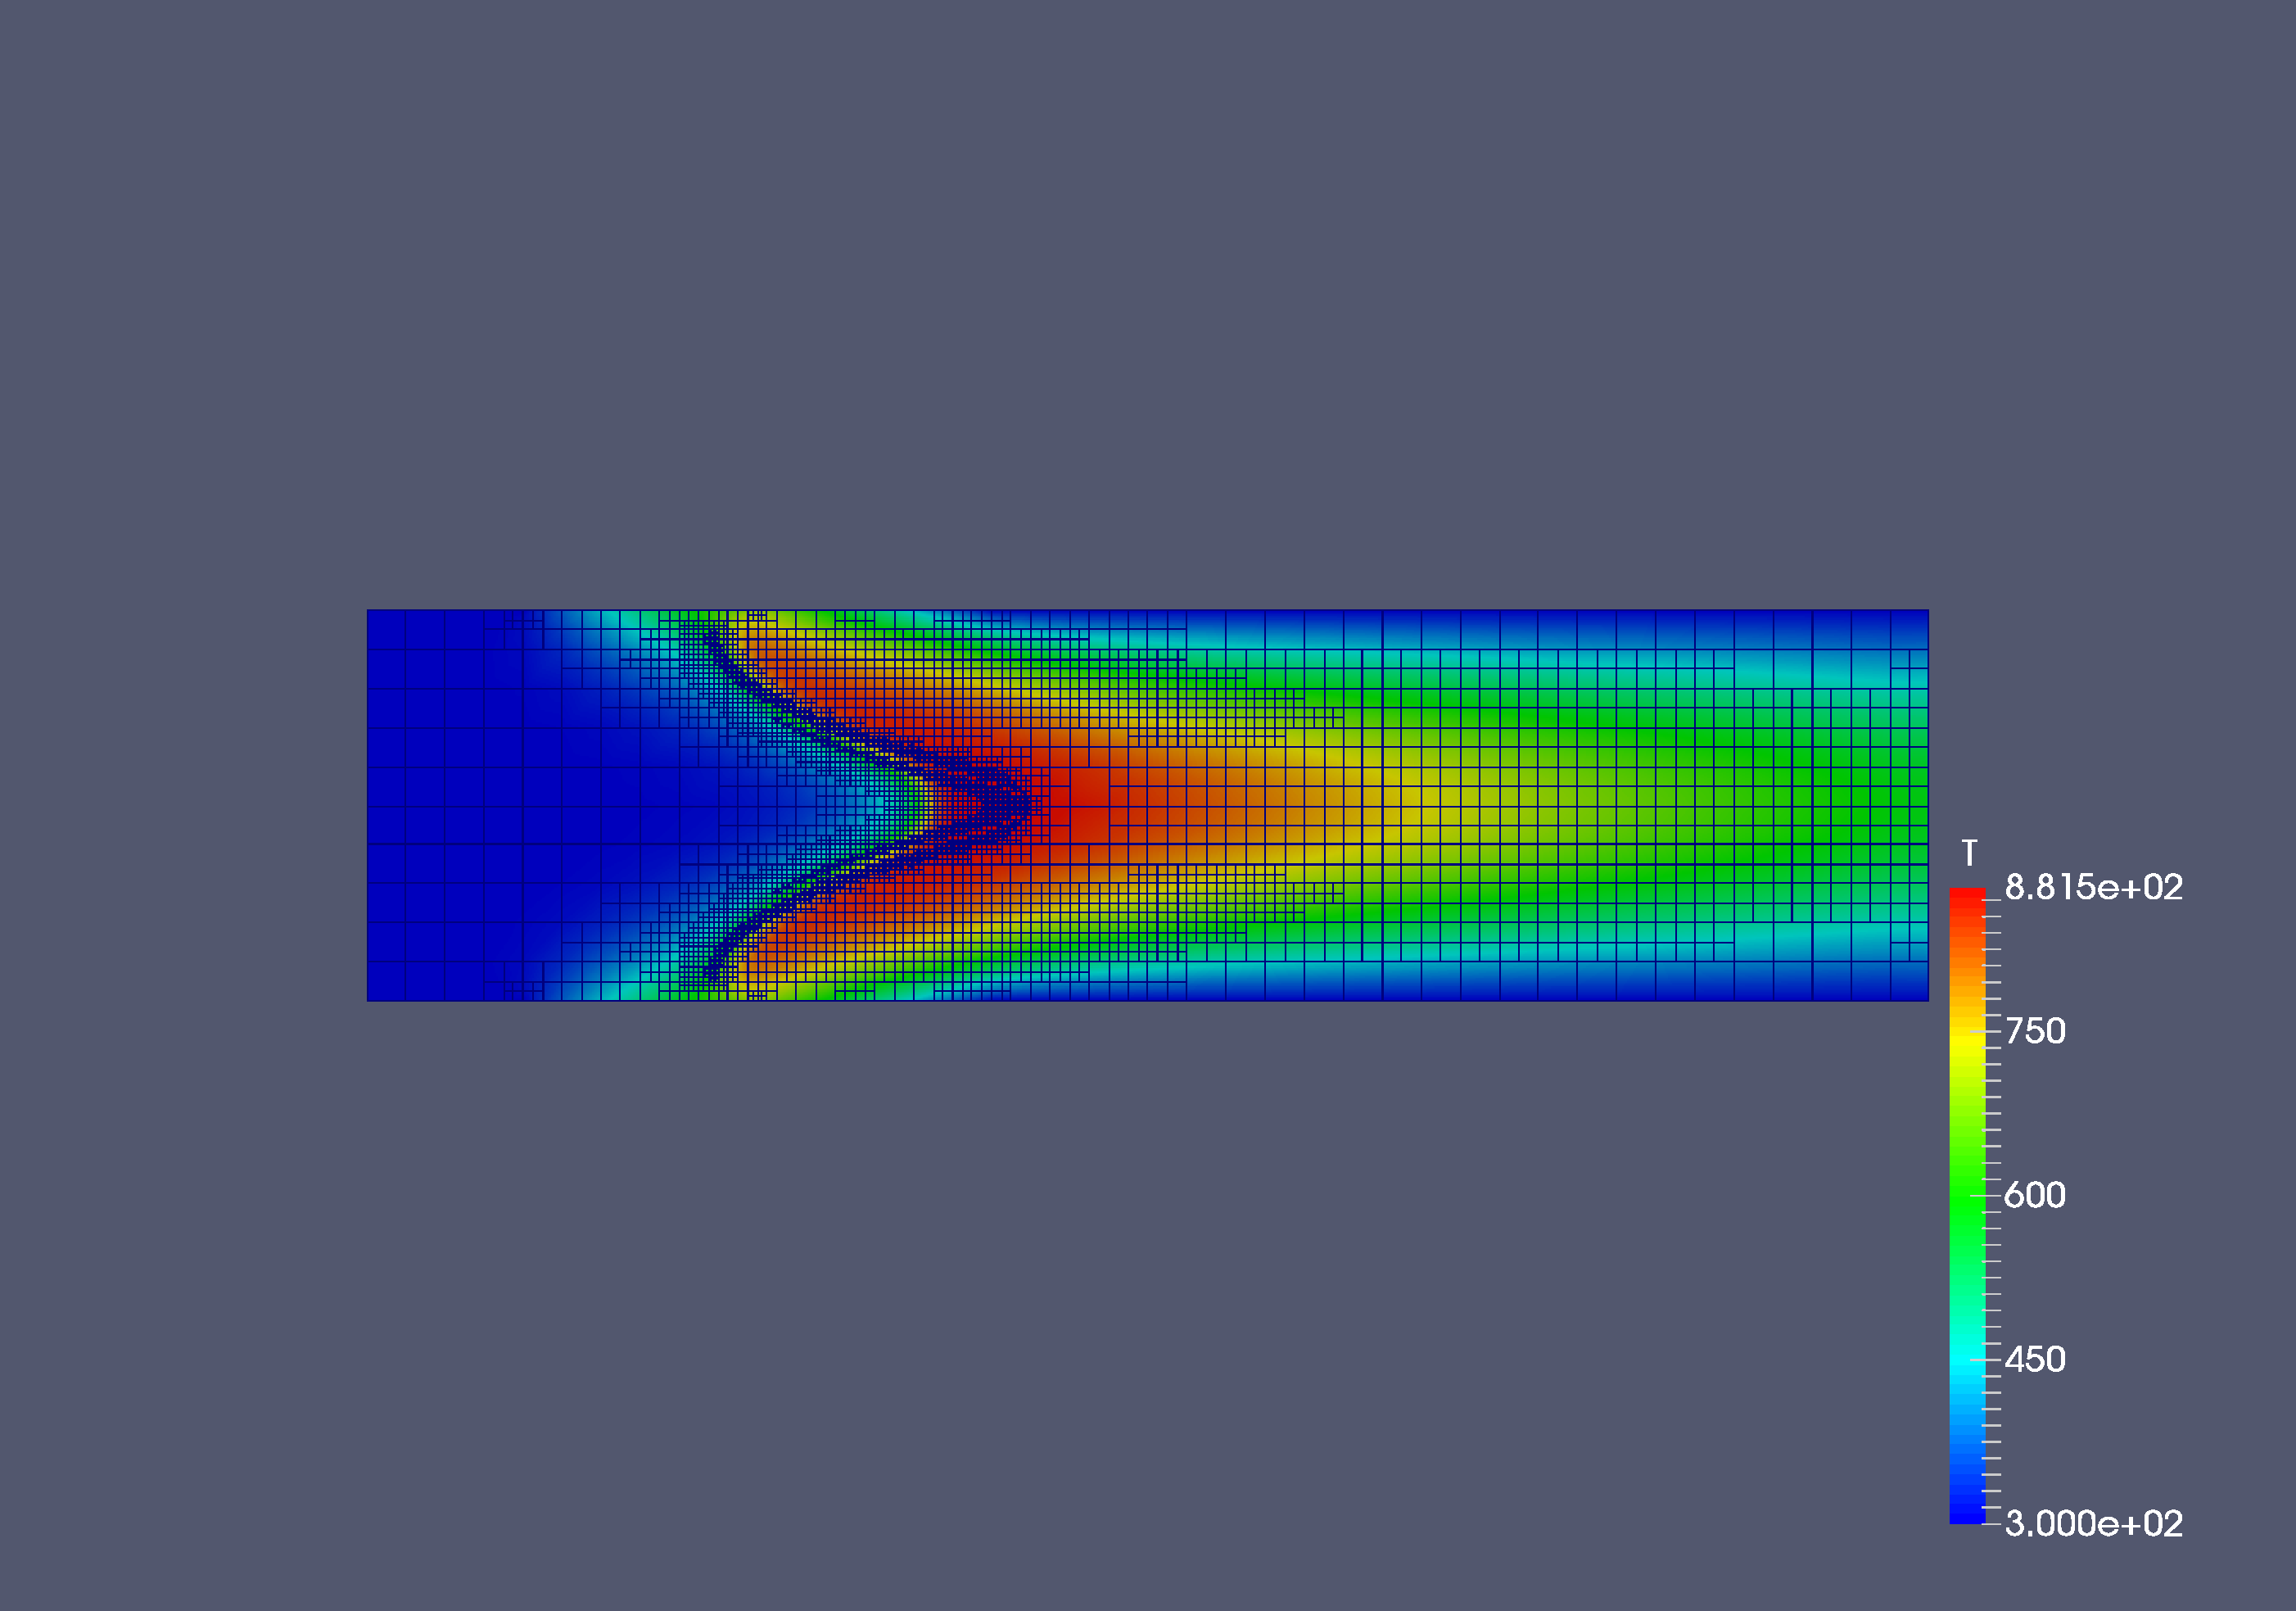
\includegraphics[scale=0.35]{figs/flame_amr.pdf}
    \caption{2D flame}
 \end{figure}

